\documentclass{article} % For LaTeX2e
\usepackage{cos424,times}
\usepackage{url}
\usepackage{graphicx}
\usepackage{hyperref}
\usepackage{subcaption}

\title{Final Project Report \\Building An Earthquake Early Warning System}


\author{
Yajun Peng\\
Department of Geosciences\\
\texttt{yajun@princeton.edu} \\
\And
Wenjie Lei \\
Department of Geosciences \\
\texttt{lei@princeton.edu} \\
}

\newcommand{\fix}{\marginpar{FIX}}
\newcommand{\new}{\marginpar{NEW}}

\begin{document}

\maketitle

\begin{abstract}
Large earthquakes can cause an immense amount of casualties and damages. To mitigate hazard in seismically active regions, we build an prototype earthquake early warning (EEW) system using machine learning approaches. We focus on southern California, and use the ground motion data from thousands of earthquakes recorded by hundreds of seismic stations. The goal is to issue fast and reliable reports of earthquake magnitudes to regions susceptible to strong ground shaking before it arrives. We test several different models including lasso regression, ridge regression, Elastic net, random forest and neural network. We show that after feature engineering, these models greatly outperform those using a few empirical measurements employed by currently operating EEW systems. We find that random forest slightly outperforms linear models. However, these models generally underestimate the magnitude of the largest earthquakes ($>$ M6). Possible reasons for this are discussed. Neural network...       

\end{abstract}

\section{Introduction}
In the past two decades, multiple devastating earthquakes occurred in densely populated regions, including the 2004 M9.2 Sumatra, 2008 M7.9 Wenchuan, 2011 M9.1 Tohoku-Oki, and 2015 M7.8 Nepal earthquakes. The resulting strong ground shaking and tsunami caused deaths of thousands of people, and property damages worth of billions of dollars. Earthquake early warning (EEW) has the potential to provide a few seconds to
a few minutes of warning before the strongest ground shaking arrives at a given
location. It takes advantage of the difference in propagation speeds between seismic and
electromagnetic waves~\cite{Allen2009, Bose2009}. The alert time can be used to adopt safety measures by individuals, to reduce train derailments, to secure chemical and radioactive materials, and to protect children in schools and patients in hospitals~\cite{Strauss2016}. Given the lack of reliable predictions for earthquake occurrences, EEW remains the primary avenue for short-term hazard mitigation. 

There are several active warning systems operating in Mexico, Japan, Taiwan, Turkey and Romania. In addition, implementation and testing of such systems are under development in United states, Europe and Asia~\cite{Allen2009, Strauss2016}. However, currently the adopted methods for EEW generally rely on empirical relations between earthquake magnitudes and several measurements derived from the recorded seismograms. Generally, the standard deviation of the prediction error in magnitude is reported to be around 0.3-0.5 unit (corresponding to a 3-6 times difference in energy release)~\cite{Bose2013}. 

In this work, we propose to explore the possibility of utilizing various machine learning techniques to obtain more reliable estimates of earthquake magnitudes. Results using previous EEW methodswould serve as the baseline.


\section{Related Work}
 The measurements often adopted in currently operating EEW systems include the predominant frequency (${tau_p}^{max}$, $tau_c$)~\cite{Allen2003, Kanamori2005} and the peak amplitude of P waves ($P_d$, $P_v$), the seismic waves that arrive first but cause weak shaking~\cite{Wurman2007}. The latter is usually corrected for the effect of geometric spreading (energy decreasing with distance). The distance-corrected $P_d$ tend to underestimate the magnitude of large earthquakes~\cite{Wurman2007}. Although ${\tau_p}^{max}$ and $\tau_c$ seem not to suffer from this, they are not very robust and often lead to a large false positive rate~\cite{Wurman2007}. These measurements will be shown in the following sections.  

\section{Methodology}
\subsection{Data Processing}
Here we focus on the southern California regions, where abundant seismicity and a dense network of seismic stations exist. Figure~\ref{stations_events} shows thousands of earthquakes with magnitude larger than 3 since 1990. There are 440 stations in total, but the number of operating stations varies with time. Therefore, we adopt the strategy of treating the recordings of an earthquake at different individual stations as independent data. We note that in practice the predictions from multiple stations can be combined to obtain a more robust estimate.   

%After training a machine learning model, we plan to use the (possibly weighted) average of the predictions from all the stations that recorded the same earthquake in question. 

\begin{figure}[ht!]
	% Requires \usepackage{graphicx}
	\centering
	\includegraphics*[scale=0.45, viewport= -20mm 40mm 500mm 230mm, angle=0]{./figure/stations_events.pdf}
	\caption{{\bf Stations (red triangles) and earthquakes (blue dots) distribution since 1990 in the study region.} For clarity, only events with magnitude larger than 3.0 are plotted.}
	\label{stations_events} %\label{figt}
\end{figure}

\begin{figure}[ht!]
	% Requires \usepackage{graphicx}
	\centering
	\includegraphics*[scale=0.75, viewport= -15mm 0mm 500mm 100mm, angle=0]{./figure/sta_lta.pdf}
	\caption{{\bf P wave arrival during a M4.17 earthquake picked by a recursive STA/LTA method.} (Upper) Seismogram at the station VTV (vertical component). A highpass filter ($>$ 1 Hz) is applied. The red line shows the P wave arrival. (Lower) Characteristic function of the recursive STA/LTA. The red dashed line shows the trigger threshold.}\label{sta_lta} %\label{figt}
\end{figure}

Data processing consists of the following steps:

\begin{enumerate}
\item Pick the P wave arrival using a standard STA/LTA algorithm~\cite{Withers1998}, which has been widely used in seismology. An example is shown in Figure~\ref{sta_lta}. 
\item Remove instrument gain such that the seismogram amplitude is within the correct range.
\item Integrate or differentiate the data as appropriate to obtain displacement, velocity and acceleration seismograms for each station.
\item Derive features from the seismograms for training linear and random forest models. Details of these features are discussed in Section 5.2.   

\item Neural network...

\item The data are divided into a training set and a test set. We find that earthquakes with magnitude larger than 4.5 constitute only 3\% of the total data volume. Since we are particularly interested in testing the predicting power on larger earthquakes, we keep in the test set 30\% of the data with magnitude $\geq$ 4.5, and 10\% of those with magnitude $<$ 4.5.

\end{enumerate}


\subsection{Methods and Evaluation Metrics}

In this project, several different well-established machine learning algorithms will be used. Since this is inherently a regression problem, we use several linear regressors (ridge, lasso, elastic net) and a tree-based method (random forest). To push our project further, we also use neural network in our prediction model. Recurrent Neural Network(RNN) has been successfully used in speech recognition, which is intrinsically similar to our problem in that both utilize the "waveforms" as input information.  We will evaluate the performance of these model with mean squared error. 

\section{Spotlight Regressor: Random Forest}

The basic idea of random forests is to build and average a collection of de-correlated trees~\cite{Breiman2001, hastie2008}. It is closely related to bootstrap aggregation or bagging. Bagging averages the prediction from models trained with bootstraped samples in order to reduce its variance. This is particularly suitable for high-variance, low-bias models, such as decision trees. If each tree can be viewed as independent and identically distributed (i.i.d) random variables with variance $\sigma^2$, then averaging $B$ such trees would result in the same expectation as the individual trees and a reduced variance $\sigma^2/B$. However, it is often likely that these trees are not independent, with pairwise correlation $\rho$, then the variance of the average is 
\begin{equation}\label{eq1}
\rho\sigma^2 + (1-\rho)\sigma^2/B. 
\end{equation}

When bagging is used, increasing $B$ would reduce the contribution from the second term, but the first term remains constant. Therefore, random forest aims to further reduce the prediction variance by decreasing the correlation between different trees~\cite{hastie2008}. This is achieved by randomly selecting a subset of all the input variables (features) for each terminal node of the tree.

The basic algorithm of random forest is as follows~\cite{hastie2008}:

For b = 1, ..., B:
\begin{enumerate}
\item Draw a sample with replacement from the training set. 
\item Train a tree model $T_b$ to the bootstrapped data. For each node of
the tree, pick the best variable among the randomly selected subset of the features, and split the node into two daughter nodes.
\end{enumerate}
For a regression problem, the prediction is the average of the predictions from the ensemble of trees (Figure~\ref{RF}):
\begin{equation}\label{eq2}
\hat{f}(x) = {1 \over B} \sum_{b=1}^{B} T_b(x) 
\end{equation}
For classification, the prediction is
\begin{equation}\label{eq3}
\hat{C}(x) = majority \ vote \{ {C_b(x)}_{b=1}^{B} \},
\end{equation}
where $C_b(x)$ is the class prediction of the $b$th tree.

Unlike many other machine learning method, quantifying generalization error or tuning hyperparameters for random forest do not require N-fold cross validation. Random forest uses out-of-bag (OOB) samples. For each observation, it constructs the predictor by averaging only those trees corresponding to bootstrap samples where the observation is not included. It can be shown that an OOB error estimate is very similar to the error obtained using N-fold cross validation. Hence, we can fit random forests in one sequence, which greatly reduces the computational expense.


\begin{figure}[ht!]
	% Requires \usepackage{graphicx}
	\centering
	\includegraphics*[scale=0.25, viewport= -170mm 0mm 500mm 190mm, angle=0]{./figure/Random_forest_prediction.png}
	\caption{{\bf A schematic illustration for the prediction process for a random forest regressor.}}\label{RF} 
\end{figure}


\section{Results Using the Baseline, Linear Models and Random Forest}

\subsection{Empirical Measurements}
In this section, we report several popular empirical measurements that have been used in literature. Figure~\ref{empirical_measurements} shows the logarithm of distance-corrected $P_d$ ($P_d * r^2$, where r is the distance from the earthquake hypocenter to the station), $\tau_c$ and $\tau_p^{max}$. 

We observe that there appears to be a quasi-linear relation between $P_d * r^2$ and magnitude. We perform a linear fit (dahsed line in Figure~\ref{empirical_measurements}), the magnitudes of large earthquakes (M $>$ 4.5) are in general underestimated. This indicates that the slope decreases with magnitude. ~\cite{Wurman2007} suggested that this might be caused by the fact that the source dimension of large earthquake is finite (not well approximated by a point). Therefore, seismic energy released by large portions of the source area may travel longer than $r$. In addition, the majority of these large earthquakes occurred before 2000, when the station distribution was very sparse. The stations were far from the earthquakes such that attenuation effect of the earth may be significant, which further reduces the seismic signal amplitude.     

\begin{figure}[ht!]
	% Requires \usepackage{graphicx}
	\centering
	\includegraphics*[scale=0.33, viewport= 40mm 0mm 500mm 120mm, angle=0]{./figure/empirical_measurements.png}
	\caption{{\bf Three empirical measurements ($P_d * r^2$, $\tau_c$, and $\tau_p^{max}$) as a function of magnitudes.}}\label{empirical_measurements} 
\end{figure}

We also observe a quasi-linear trend for $\tau_c$ and $\tau_p^{max}$ for earthquakes larger than M4. However, the significant scatter for the smaller earthquake excludes the possibility of achieving good predicting performance using a simple linear fit. This is consistent with findings in previous studies~\cite{Wurman2007}. Hence, in the following sections, we use only the linear fit for $P_d * r^2$-magnitude as the baseline.  


\subsection{Linear Models and Random Forest}
\subsubsection{Feature Engineering}
To train machine learning models, we wish to incorporate features other than few popular empirical measurements (Figure~\ref{empirical_measurements}). Here only broadband velocity seismograms are used. The velocity records are then integrated to displacement and differentiated to acceleration. We also make velocity envelopes. Each of these four types of records has three components (east, north, and vertical). For each component, we use 0.5, 1, 1.5, ... to 3-second time windows since the arrival time picked by the STA/LTA algorithm Figure~\ref{sta_lta}. For each time window, we compute the maximum, the relative time within a window for the maximum, mean, variance, skewness, kurtosis, percentile (0.25, 0.5, 0.75), and norm (L1, L2, L4), $\tau_c$ and $\tau_p^{max}$. The distance from the earthquake hypocenter to the station ($r$) is also included. We have in total 1663 features. We note there may be many redundant features, especially for amplitude information. It is possible that the performance could be improved if we incorporate more frequency-related features. But currently we use only $\tau_c$ and $\tau_p^{max}$. For random forest, the amplitude-related features are corrected by the earthquake-station distance. Most of these features are transformed into the logarithmic scale. Exceptions include skewness and kurtosis. 
\subsubsection{Prediction Performance}
We use 5-fold cross validation to tune the hyperparameters for the linear models (lasso, ridge, elastic net), and out-of-bag scores for random forest. Then the models are used to predict the earthquake magnitudes in the test set.

The evaluation metrics for the regressors are shown in Table~\ref{tab1}. All the machine learning methods outperform the baseline, with random forest being slight better than the linear models. This may suggest a weak non-linear relation between the features and the magnitudes. As expected, the lasso regression and elastic-net regression produce the most sparse models, with only 347 and 349 features with non-zero coefficients (linear models) or importance (random forest).   

\begin{table}[htbp]
	\small
	\centering
	\begin{tabular}{@{}|c|c|c|c|c|c|@{}} % Column formatting, @{} suppresses leading/trailing space 
		\hline
%		&  \multicolumn{4}{c}{No feature selection} &
%		\multicolumn{4}{c|}{Feature selection}  \\
		\cline{2-4}
		Regressor & MSE & MSE ($<$ M4.5) & MSE ($\geq$ M4.5) & Mean error ($\geq$ M4.5) & Non-zero features\\ \hline \hline
		Baseline & 0.0899 & 0.0695 & 0.2620 & -0.4250  & 1 \\
		RF & 0.0451 & 0.0388 & 0.0981 & -0.1536 & 1663 \\ 
		Lasso &  0.0565 & 0.0477 & 0.1309 & -0.2470 & 347 \\ 
		Ridge & 0.0560 & 0.0477 & 0.1260 & -0.2421 & 1663 \\ 
		EN & 0.0565 & 0.0476 & 0.1310 & -0.2470 & 349 \\ \hline
	\end{tabular}
	\caption{{\bf Results from the adopted regressors on the test set.} The first three columns show mean squared error (MSE) for the whole test set, the small earthquakes ($<$ M4.5) and the large earthquakes ($\geq$ M4.5). The mean error for large earthquakes and the number of features with non-zero coefficients (linear models) or importance (random forest) are also reported.}
	\label{tab1}
\end{table}

Figure~\ref{prediction_vs_true} shows the predicted magnitudes and error compared to the true magnitudes. As mentioned in Section 5.1, the baseline model systematically underestimates the magnitudes of large earthquakes. For lasso and random forest models, this effect is less severe. However, it seems that even using the latter two models, we still underestimate the magnitudes of the large earthquakes ($geq$ M4.5), as shown by the mean error (Table~\ref{tab1}). The MSE for the small earthquakes is several times less than that of the large earthquakes. At least one of the reasons is that the number of samples within this magnitude range is too small. Another reason could be that there are not many features which are not sensitive to the finite fault effect for large earthquakes, such as reliable frequency-related features.      




\begin{figure}[ht!]
	% Requires \usepackage{graphicx}
	\centering
	\includegraphics*[scale=0.18, viewport= 85mm 40mm 800mm 460mm, angle=0]{./figure/prediction_vs_true.png}
	\caption{{\bf Predictions by the baseline model, linear models (lasso, ridge, elastic net), and random forest.} The three rows show the train set, the test set, and the test error respectively. The dashed lines show zero error.}\label{prediction_vs_true} 
\end{figure}




\subsubsection{Important features}
Figure~\ref{Feature_importance_lasso_RF} shows the most important features for lasso and random forest. It is expected that distance would be very important for lasso but not for random forest because the amplitude-related features for the former are not corrected for geometrical spreading (distance). It seems that all but one for random forest are derived from the vertical component of the displacement time series (labeled as BHZ.disp), while features for lasso show a greater variety. This seems consistent with that the signal-to-noise ratio for P wave is generally higher for the vertical component, but there could be some non-linearity that may not be fully explained by a linear model such as lasso. In addition, frequency-related features are more important for lasso (e.g. $\tau_c$).  

\begin{figure}[ht!]
	% Requires \usepackage{graphicx}
	\centering
	\includegraphics*[scale=0.5, viewport= 12mm 0mm 500mm 120mm, angle=0]{./figure/Feature_importance_lasso_RF.pdf}
	\caption{{\bf Top 20 most important features for lasso regression and random forest.} In the random forest model, distance has been corrected for, although it is also kept as a feature. Therefore, the importance of distance is expected to be not as high as in lasso.}\label{Feature_importance_lasso_RF} 
\end{figure}


\section{Neural Networks and LSTM}
Neural networks are famous for its function of "automatic feature extraction". So for the input layer, instead of using empirical features, we tried used several "raw" measurements, including the time series of displacement, velocity, acceleration and cumulative acceleration of the ground motion. As we have mentioned in the linear models, we cropped 3 seconds window starting from the onset, which give us total 60 data points, given the sampling rate of instrument is 20Hz on one component. Since in total we have three components data, plus the distance information, the input layer size is $3*60 + 1 = 181$. 

Again, considering the symmetrical feature of input, i.e., given the sign reverted ground motion, it ends up with same magnitude of earthquakes, we did one more step, using the envelope transition, rather than the raw waveform, as the features of input layer. To avoid over-fitting, we include the $\l2$ regularization and a dropout layer.

\subsection{Hyper-parameter tuning using validation dataset}
The \textbf{hyper-parameter} in Neural networks includes the \textbf{number of hidden layers}, the \textbf{number of neurons in each hidden layers}, the learning rate, weight decay($l2$ regularization coefficient), dropout ratio, the activation function and so on. Due to the high cost of training a neural network, here we only focusd on tunning two parameters, the number of hidden layers and the number of neurons in each hidden layers, which affect the representation capability of neural networks the most. For the layout of neural networks, we keep the number of neurons the same in each hidden layer.

For the choice of activation function, we tried using ReLU and Tanh. It turns out that the \textbf{ReLU} gives much better performance, from the point view of convergence rate and final loss values. As for other parameters, we set the weight decay to 0.005, the drop ratio to 10\%.



\begin{table}[htbp]
	\small
	\centering
	\begin{tabular}{@{}|c|c|c|c|c|c|c|@{}} % Column formatting, @{} suppresses leading/trailing space 
		\hline
%		&  \multicolumn{4}{c}{No feature selection} &
%		\multicolumn{4}{c|}{Feature selection}  \\
		%\cline{2-7}
		Neurons in each layer & 10 & 20 & 50 & 100 & 180 & 300\\ 
		\cline{1-7} \hline \hline
		hidden layer = 1 & 0.1098 & 0.1476 & \textbf{0.1130} & 0.1046  & 0.1092 & 0.1159 \\
		
		hidden layer = 2 & 0.0895  & \textbf{0.0872} & 0.0915 & 0.0978 & 0.0899 & 0.0873 \\ 
		hidden layer = 3 &  0.0994 & 0.0950 & 0.1479 & \textbf{0.0861} & 0.0906  & 0.0942 \\ 
		 hidden layer = 5 & 0.0883 & 0.1128 & 0.0865 & 0.0947 & \textbf{\underline{0.0862}}  & 0.0990\\ 
		 hidden layer = 10 & 0.0944 & 0.0948 & 0.0935 & 0.0912 & \textbf{0.0878} & 0.2084  \\ \hline
	\end{tabular}
	\caption{{\bf MSE values on the validation data using different number of hidden layers and neurons in each hidden layer, using 25 epoch for training.} The best performance is given by the model (hidden\_layers=5, neurons=180), which is underlined in the table.}
	\label{tab:nn_cv}
\end{table}

In order to tune the hyper-paramters, we split the train data one step more, keeping 80\% as train data and 20\% as validation data. Table\ref{tab:nn_cv} shows our validation results, using the displacement as the input feature. From the table, we can see that there is really no clear patterns as to set the number of layers and neurons, indicating the complexity and non-linearity of neuron networks. One observation, though, coming from the table, is that setting the number of neurons in each hidden layer to 300, might there is no optimal models coming from that setting. Since our input layer is in dimension of 181, 300 might leads to over-fitting our model.  On the other hand, setting the number of neurons to 10 is might also leads to under-fit.

\subsection{Long Short-Term Memory(LSTM)}
We also tried LSTM here since our input feature is basically time series. However, the MSE of validation and test data, stays around 0.180 and won't reduce any more. We got one model, using the acceleration as input time series, reaches the MSE value as 0.140. However, the MSE value is still way beyond our baseline mode. One difficulty we found in LSTM is there a very important feature, distance, very difficulty to incorporate into the LSTM framework since it doesn't have any temporal relationship with the time series. Unlike the task of speech recognition, in which the shape of waveform is important but the absolute amplitude is not, distance will play a vital role in prediction the magnitude since the amplitude of  waveform will decay in exponential order with distance.


\subsection{Performance Summary}

\begin{table}[htbp]
	\small
	\centering
	\begin{tabular}{@{}|c|c|c|c|c|c|c|@{}} % Column formatting, @{} suppresses leading/trailing space 
		\hline
%		&  \multicolumn{4}{c}{No feature selection} &
%		\multicolumn{4}{c|}{Feature selection}  \\
		\cline{2-6}
		Input features & MSE & MSE($<$M4.5) & Mean Error($<$M4.5)& MSE($\geq$M4.5) & Mean Error($\geq$M4.5)\\ 
		\cline{2-6} \hline \hline
		displacement & \textbf{\underline{0. 0861}} & \textbf{0.0839} & 0.0739 & \textbf{0.1920}  & \textbf{-0.2258} \\
		 velocity & 0.1040  &  0.0981 & 0.1204 & 0.2566 & -0.3206\\ 
		acceleration &  0.1022 & 0.0963 & 0.1056 & 0.2500 & -0.3061 \\ 
		 cumul acc & 0.0991 & 0.0915 & \textbf{0.0434} & 0.2876  & -0.2979 \\ 
		 LSTM & 0.1410 & 0.1162 & 0.0981 & 0.7011 & -0.7329 \\
		 \hline
	\end{tabular}
	\caption{{\bf The MSE values of Neural networks using different input features.} The best performance is given by the model (hidden\_layers=5, neurons=180), which is underlined in the table.}
	\label{tab:nn_perf}
\end{table}

From table\ref{tab:nn_perf}, we can see that the overall performance of Neural networks beats the baseline model but still not as good as linear models or random forest. What is more, the under-estimation of large events, which is measured by the mean error in the table, is also reduced compared to linear models, though the difference is not significant. The LSTM model doesn't achieve very good results in our current settings. Originally, we thought LSTM is the best method when dealing with time series data. However, due to special settings of our problem, that we need to incorporate distance information, it turns out it needs more tunnings in the future.

In summary, the Neural network beats the baseline model and out-performs linear model in some aspects but it is still not good as Random Forest.  The LSTM needs more work in the future.

\begin{figure}[ht!]
\centering
\begin{subfigure}{0.48\textwidth}
\centering
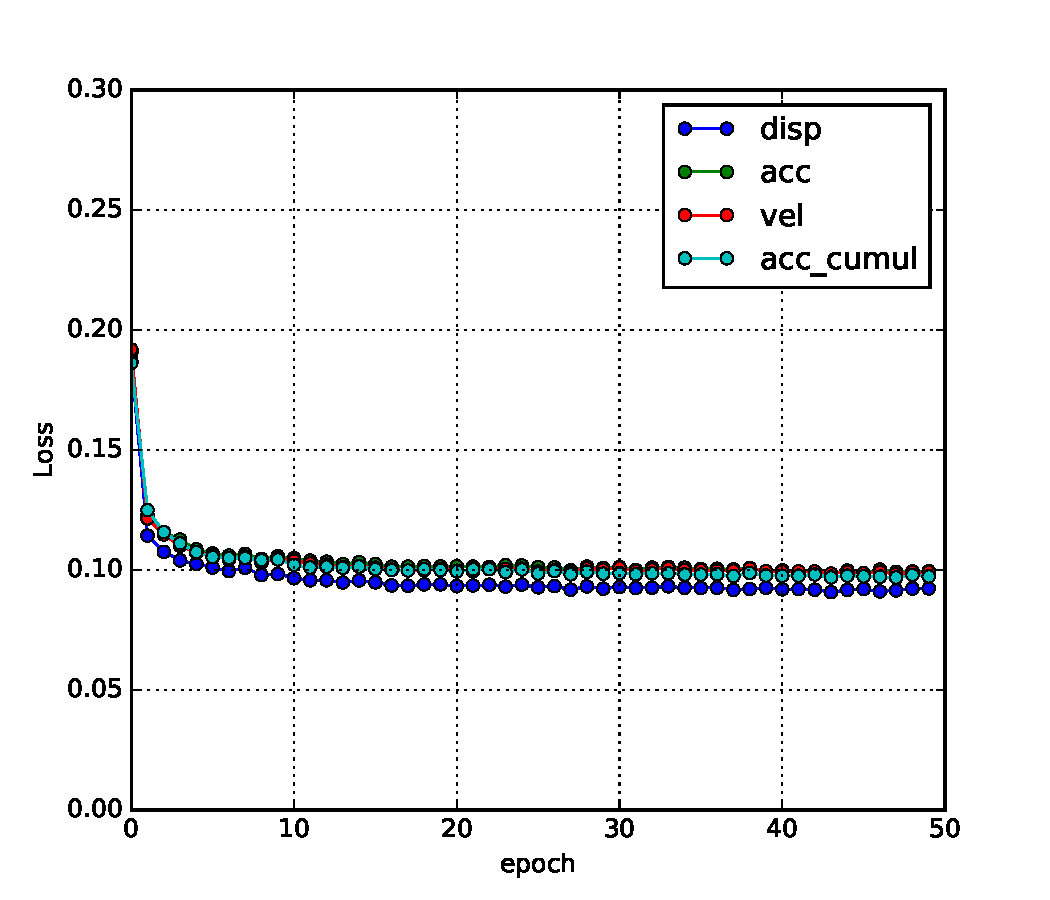
\includegraphics[width = \textwidth]{./figure/nn_loss}
\caption{variance explained by singular values}
\label{fig:svd_left}
\end{subfigure}
\begin{subfigure}{0.48\textwidth}
\centering
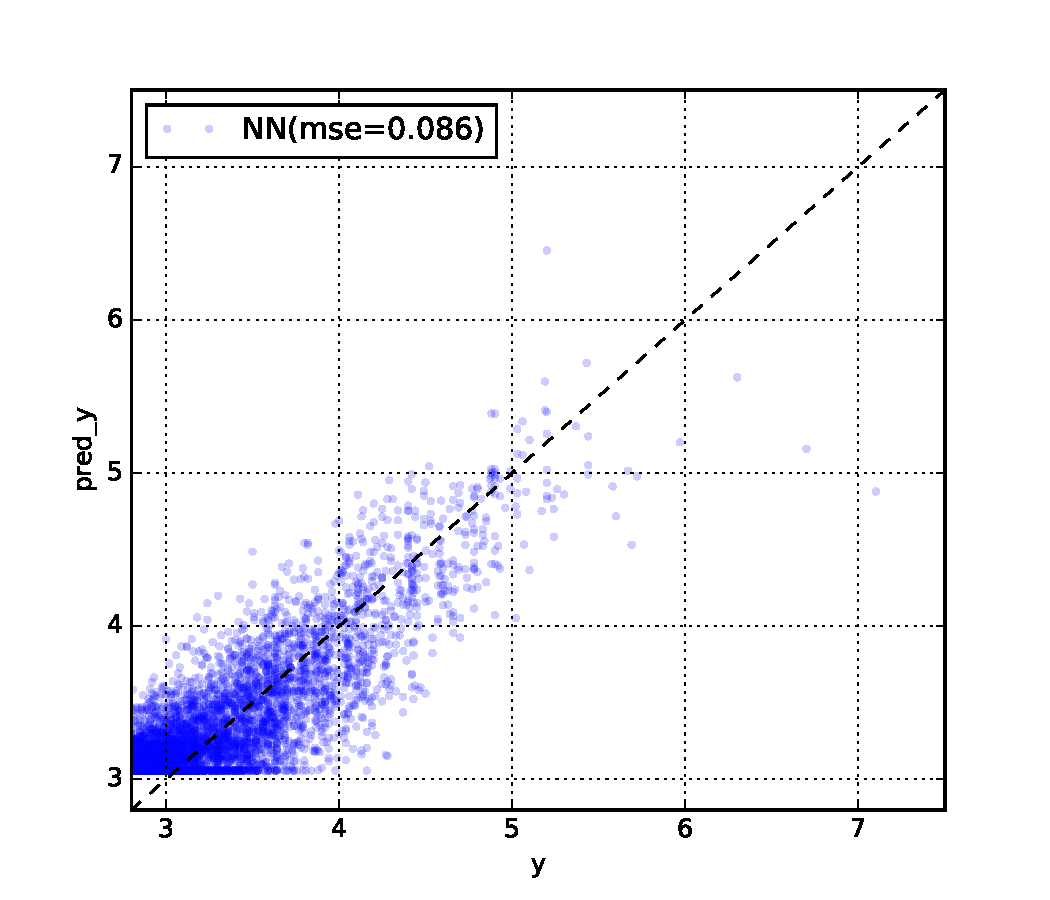
\includegraphics[width = \textwidth]{./figure/nn_prediction}
\caption{The voilin plot of probabilities}
\label{fig:svd_right}
\end{subfigure}
\caption{Training and prediction results from Neural Network. The figure on the left shows change of loss(mean squared error) with epoch in the training procedure, with different features as the first input layer. The figure on the right shows the prediction magnitudes versus the true magnitudes.}
\label{fig:combined}
\end{figure}

\section{Discussions and Conclusions}

%\section{Scientific Questions}
%Although the primary goal of this proposal is to reduce the error in fast, real-time report of earthquake magnitudes, we hope that the results could also shed light on several important scientific questions that are yet to be resolved in seismology. These include: (1) Is there enough information in the first a few seconds of the seismograms to predict the final magnitude of an earthquake? If yes, what is it? The answer to this would be very important for decreasing the size of ``blind zone" during an earthquake (the region that the strong shaking arrives before the warning is issued); (2) Is there self-similarity across earthquakes with a wide range of magnitudes? Small earthquakes (less than M5) occur much more frequently than large earthquakes; the former dominates our dataset. Can we use small earthquakes to infer the properties of large earthquakes? (3) Is it possible to reduce the number of false positives in our system, which trigger alarm without real earthquake happening and cause unnecessary panic? To address these questions would have not only substantial societal impact, but also significant implications for understanding earthquake dynamics.    


%\subsubsection*{Acknowledgments}

\newpage
\bibliography{ref}
\bibliographystyle{plain}

\end{document}
